\chapter{Einführung und Wiederholung}{\label{ch:intro}}
Dieses Kapitel stellt eine Einführung in die erweiterte Maßtheorie dar. Es setzt dabei einen geübten Umgang mit der Maß- und Integrationstheorie, sowie der Funktionalanalysis voraus. Da die Variationsrechnung keine Standardvorlesung darstellt, werden hierfür in \ref{sec:calcvar} die wichtigsten Grundlagen zusammengetragen. Abschließend erfolgt ein Einstieg in die Theorie der beschränkten Variation (\(\mathcal{BV}\)-Theorie), da diese bei weitem keine übliche Vorlesung darstellt.\\
Im Folgenden setzen wir dann fest:
\begin{itemize}
    \item \(n,m,N \in \mathbb{N}\),
    \item \(\epsilon > 0\).
\end{itemize}
%%%%%%%%%%%%%%%%%%%%%%%%%%%%%%%%%%%%%%%%%%%%%%%%%%%%%%%%%%%%%%%%%%%%%%%%%%%%%%%%%%%%%%%%%%%%%%%%%%%%%%%%%%
\section{Maßtheoretische Grundlagen}{\label{sec:measure}}
Wir erinnern uns kurz zurück an die Grundlagen der Maßtheorie und setzen hierbei fest, dass wir mit (hierbei sei stets \(A \subset \mathbb{R}^n\)):
\begin{itemize}
\item
    \(\mathcal{B}(\mathbb{R}^n):=\mathcal{B}(\mathbb{R}^n,\mathcal{T}_{ecl}) := \sigma(\mathcal{T}_{ecl})\),
\item
    \(\mathcal{M}^n(A) : = \{B \in \mathcal{B}(\mathbb{R}^n) \, | \, B \cap A \in \sigma(E)\}\), wobei \(E \subset \mathcal{T}_{sub}\),
\item
    \(\lambda^n: \mathcal{B}(\mathbb{R}^n) \to [0,\infty] \text{ mit } \lambda^n(\bigtimes_{i=1}^n ]a_i,b_i]) = \prod_{i=1}^n |b_i - a_i| \, \, \forall a, b \in \mathbb{R}^n\),
\item
    \(\mathcal{H}^n(A) := \lim_{\epsilon \to 0^+} \inf \{\sum_{i=1}^{\infty} (\text{diam }U_i)^n \, | \, U_i \subset \mathbb{R}^n, \, \bigcup_{i=1}^{\infty} U_i \supseteq A, \text{ diam }U_i < \epsilon \}\),
\end{itemize}
die Borelsche \(\sigma\)-Algebra im \(\mathbb{R}^n\), dessen Elemente man Borelmengen nennt, die \(\sigma\)-Algebra aller messbaren Teilmengen im \(\mathbb{R}^n\), das n-dimensionale Lebesgue-Maß und das n-dimensionale Hausdorff-Maß meinen.\\
Um viele der variationellen und stochastischen Problemstellungen dieser Arbeit \\allerdings analytisch untersuchen zu können, ist das Lebesgue-Maß zu restriktiv oder sogar komplett ungeeignet. Letzteres ist der Fall, wenn wir Funktionen der Form:
\begin{equation}{\label{eq2.1}}
f:B \to [0,\infty],\text{ wobei }(B,||\cdot||) \text{ Banach, \(\infty\)-dimensional und seperabel}
\end{equation}
betrachten. Es gilt allgemein:\\[0.5cm]
\pgfsetfillopacity{0.1}\colorbox{generalYellow}{\begin{minipage}{16cm}{\textcolor{black}{\pgfsetfillopacity{1}}{\label{theo2.1}}}
\textbf{Satz 2.1 (Eigenschaften des Lebesgue-Maßes, \cite{ElstrodtMeas}[Seite 100: 2.1 Satz, Seite 74: 7.2 Korollar, Seite 73-74: 7.1 Satz]):} Betrachte den Maßraum \((X,\mathcal{B}(\mathbb{R}^n),\mu)\). \\
Ist \(X=\mathbb{R}^n, \, \mu = \lambda^n\) dann:
\begin{enumerate}
    \item \(\lambda^n(A+x) = \lambda^n(A) \, \forall x \in \mathbb{R}^n \, \forall A \in \mathcal{B}(\mathbb{R}^n)\). (\textbf{Translationsinvarianz})
    \item \(\lambda^n(A) = \sup \{\lambda^n(K) \, | \text{ K ist ein Kompaktum in A}\} \, \forall  A \in \mathcal{B}(\mathbb{R}^n)\). (\textbf{Innere Regularität})
    \item \(\forall x \in \mathbb{R}^n \, \exists \text{ Umgebung } U \in \mathcal{B}(\mathbb{R}^n)\):\(\, \lambda^n(U) < \infty\). (\textbf{Lokale Endlichkeit})
\end{enumerate}
Ist \(X\) der Banachraum B aus \eqref{eq2.1}, gilt jedoch:\\
Erfüllt \(\mu\) die drei eben aufgeführten Eigenschaften für B, so ist \(\mu(A)=0\) für alle Borelmengen A.
\end{minipage}}\\

\textsc{Beweis:} Für den \(\mathbb{R}^n\)-Fall verweisen wir auf die angegebenen Quellen. Die Banachraum-Verallgemeinerung ist ein Korollar aus dem wohlbekannten Riesz-Lemma (siehe z.B. \cite{brezis2011functional}[Seite 160: Lemma 6.1 (Riesz's lemma)]).\QEDB

\textbf{Bemerkung:} Erfüllt ein nicht-negatives Maß [\ref{theo2.1}, Satz 2.1 (2),(3)], so nennt man dieses ein Radon-Maß.\\

Wir wollen wie angekündigt das Lebesgue-Maß/-Integral sinnvoll (!) verallgemeinern. Wir führen nun Vektor-(Radon-)Maße und das Bochner-Integral ein:\\[0.5cm]
\pgfsetfillopacity{0.1}\colorbox{generalYellow}{\begin{minipage}{16cm}{\textcolor{black}{\pgfsetfillopacity{1}}{\label{def2.2}}}
\textbf{Definition 2.2 (Vektor-(Radon-)Maße und Bochner-Integral):} Sei \(\RK\) der Raum der relativ-kompakten Mengen \(A \subseteq \mathbb{R}^n\). Dann definieren wir:
\begin{enumerate}
    \item Für einen Maßraum \((A,\mathcal{B}(A),\mu)\) mit \(\mu : \mathcal{B}(A) \to \mathbb{R}^N\) nennen wir \(\mu\) ein Vektor-Maß auf A, falls dieses abzählbar additiv ist. Den zugehörigen Raum bezeichnen wir mit \(\mathcal{M}(A,\mathbb{R}^N)\).
    \item Gilt für \(\nu: \RK \to \mathbb{R}^N\):
    \begin{equation}
    \begin{array}{l}
        \exists \text{ nicht-negatives Radon-Maß } \mu \text{ auf A } \exists \, f \in L^1_{loc}(A,\mu): \\ 
        \, \nu(A) = \int_{A} f\, d\mu \, \, \forall A \in \RK,
    \end{array}
    \end{equation}
    dann nennen wir dieses ein Vektor-Radon-Maß auf A. Analog zu (1) \\bezeichnen wir den zugehörigen Raum mit \(\RM\). Ist N=1, so spricht man von einem signierten Maß.
    \item Für allgemeine Abbildungen \(f: \mathbb{R}^n \supseteq \Omega \to \mathcal{B}\), mit \(\mathcal{B}\) einem Banachraum, definieren wir analog zum Lebesgue-Integral das sogenannte Bochner-Integral auf einem \(\sigma-\)endlichen und vollständigen Maßraum \((\Omega,\Sigma_{\Omega},\mu)\) durch:
    \begin{equation}
        \forall \text{ disjunkten } B_i \in \Sigma_{\Omega}: \int_{\Omega} f \, d\mu := \int_{\Omega} (\sum_{i=1}^n \chi_{B_i}x_i) d\mu := \sum_{i=1}^n \mu(B_i)x_i .
    \end{equation}
\end{enumerate}
\end{minipage}}

\begin{figure}[label={fig:boch}, caption={Illustration des Bochner-Integrals \cite{RelaxPaper}}]
    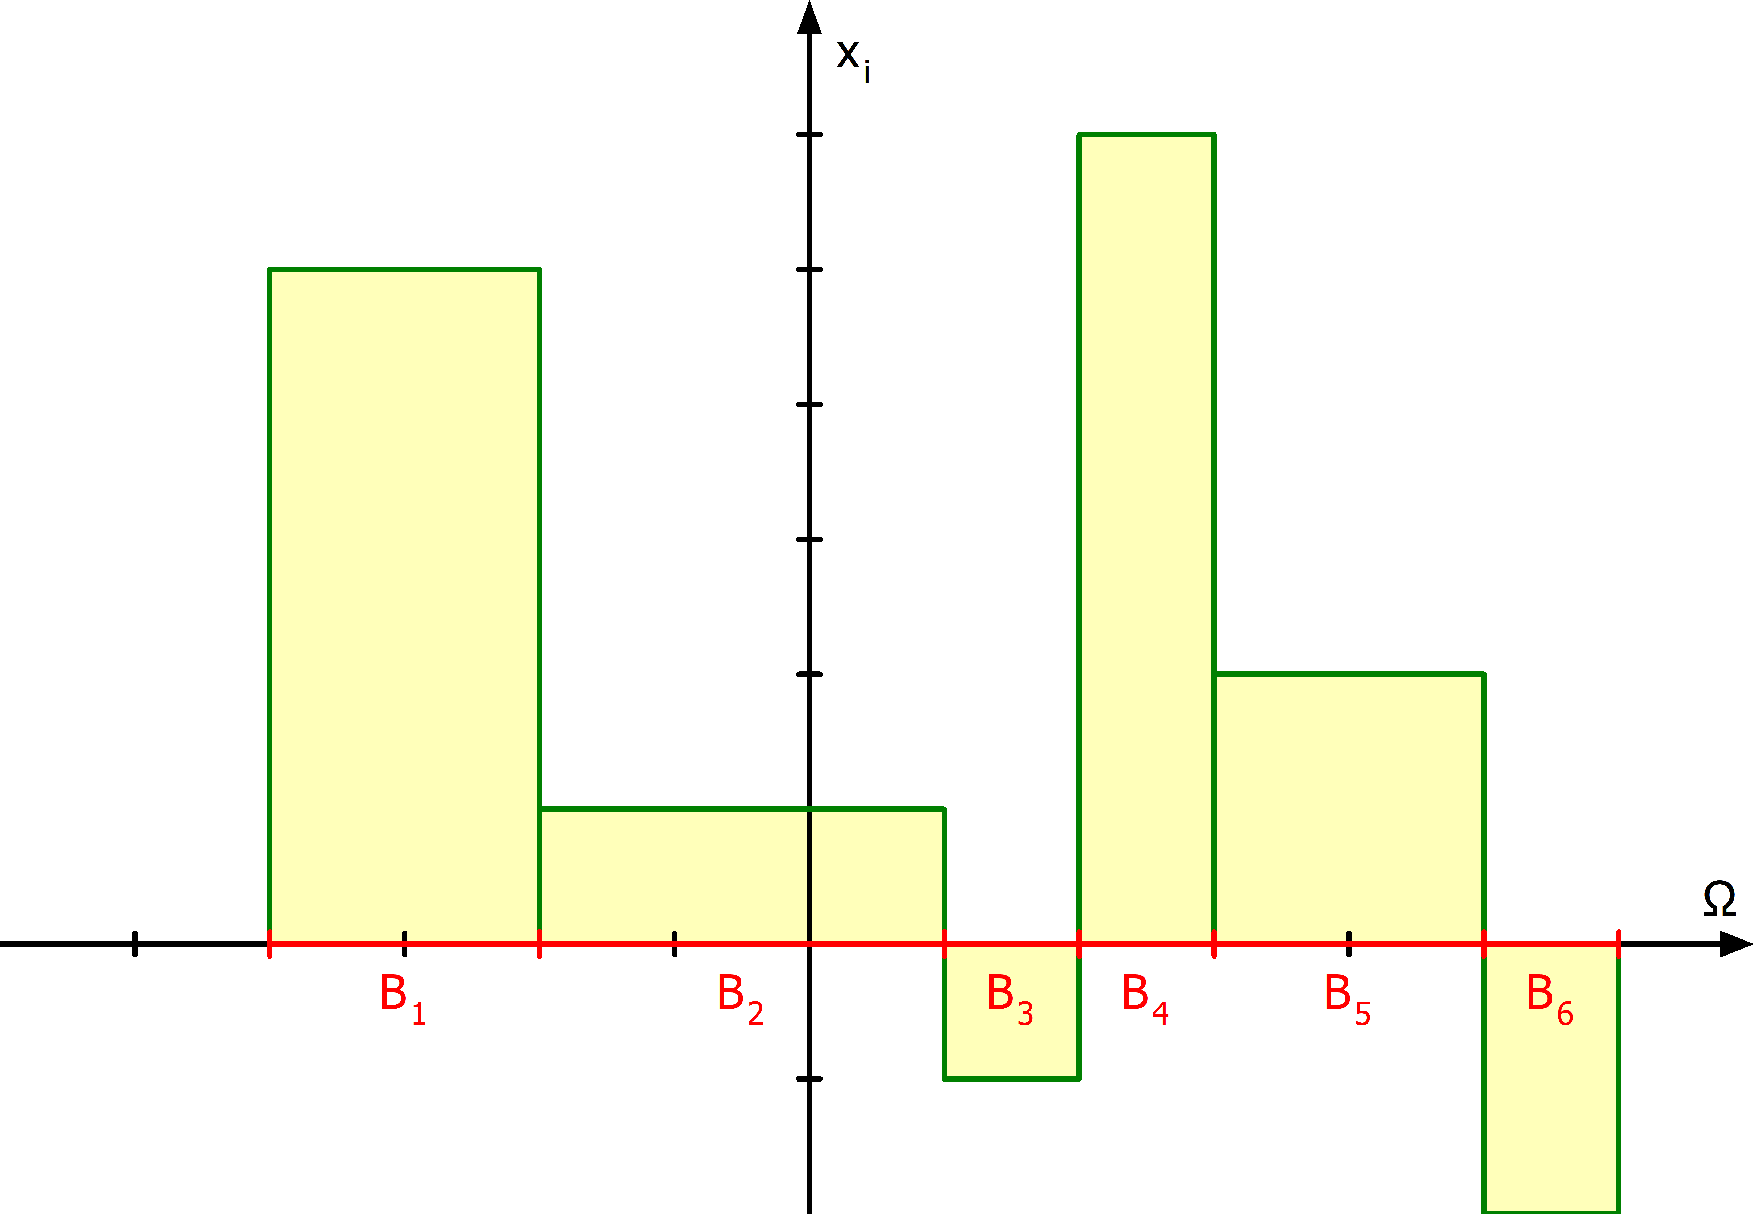
\includegraphics[scale=0.4]{figures/BochnerOhneUrsprungPDF.pdf}
\end{figure}

\textbf{Bemerkung:} Der Raum \(\RK\) ist nötig für [\ref{def2.2}, Definition 2.2 (2)], da sonst nicht-definierte Unendlichkeitsausdrücke auftreten könnten.\\

Sehr wichtig für die Analysis von Sobolevfunktionen sind sogenannte Lebesgue-Punkte. Dass diese überhaupt existieren, liegt an folgendem Lemma:\\[0.5cm]
\pgfsetfillopacity{0.1}\colorbox{generalYellow}{\begin{minipage}{16cm}{\textcolor{black}{\pgfsetfillopacity{1}}{\label{lem2.3}}}
\textbf{Lemma 2.3 (Besicovitch):} Betrachte \(\nu \in \M, \, \mu\) ein nicht-negatives, signiertes Maß auf A und ein \(f \in L^1(A,\mu,\mathbb{R}^N)\). Stellen nun f und \(\mu\) die Radon-Nikodym-Zerlegung von \(\nu\) dar (i.e. \(\nu = f\mu + \nu_s\)), dann existiert \(\mu\)-f.ü. für \(x \in \text{ supp }\mu\) die folgende Beziehung zwischen Radon-Nikodym-Ableitung und dessen Limes:
\begin{equation}
    f(x) = \frac{d\nu}{d\mu}(x) = \lim_{\epsilon \to 0^+} \frac{\nu(B_{\epsilon} (x))}{\mu(B_{\epsilon}(x))} =: d\nu^+.
\end{equation}
\end{minipage}}\\

\textsc{Beweis:} Das Lemma stellt eine alternative Variante des wohlbekannten Satzes von Radon-Nikodym dar und benutzt für den Beweis entscheidend folgendes Lemma:\\
Sei \(0 < \alpha < \infty\). Dann gilt:
\begin{equation}
    (A \subset \{x \in \mathbb{R}^n \, | \, d\nu^+ \leq \alpha \} \, \Rightarrow \, \nu(A) \leq \alpha \mu(a)).
\end{equation}
Für weitere Details verweisen wir auf \cite{EvansMeaTh}[Seite 37-44].\QEDB

\textbf{Bemerkung:} Der Satz von Radon-Nikodym (zusammen mit dem Zerlegungssatz von Hahn) impliziert ein weiteres wichtiges Theorem für die Maßtheorie, nämlich den Jordanschen Zerlegungssatz:\\
Für alle \(\mu \in \M\) existiert eine Jordan-Zerlung \(\mu = \mu^+ - \mu^-\) mit \(\mu^{\pm}:=f^{\pm}|\mu|, \\f \in L^1(A,|\nu|,\mathbb{R}^N)\).\\
Diese Jordan-Zerlegung findet insbesondere Anwendung im Beweis des obigen Lemmas [\ref{lem2.3}, Lemma 2.3].\\

Nun befinden wir uns also in der Situation, festzuhalten, was wir unter Lebesgue-Punkten verstehen:\\[0.5cm]
\pgfsetfillopacity{0.1}\colorbox{generalYellow}{\begin{minipage}{16cm}{\textcolor{black}{\pgfsetfillopacity{1}}{\label{def2.4}}}
\textbf{Definition 2.4 (Lebesgue-Punkte):} Sei \(\mu\) ein nicht-negatives signiertes Maß auf A, \(f \in L^1(A,\mu)\). Erfüllt \(x \in \text{ dom }(f)\) die Bedingung:
\begin{equation}
    \lim_{\epsilon \to 0^+} \intbar_{B_{\epsilon}(x)} |f(x)-f(y)| \, d\mu(y) = 0
\end{equation}
für \(\mu = \lambda^n\), so nennen wir x einen Lebesgue-Punkt (für f).
\end{minipage}}\\

\textbf{Bemerkung:} \begin{itemize}
    \item Nach [\ref{lem2.3}, Lemma 2.3] existieren solche x natürlich auch für alle anderen nicht-negativen signierten Maße auf A. Es wird nur der wichtige Spezialfall des Lebesgue-Maßes mit Lebesgue-Punkten notiert.
    \item Allgemein wird bekanntlich etwas informell in \(L^p\)-Räumen nicht zwischen \\Äquivalenzklasse und Funktion unterschieden - mit Ersterem den eigentlichen Elementen dieses Funktionenraumes. Für die Menge der Lebesgue-Punkte ist es aber entscheidend, welcher Repräsentant gewählt wird.
\end{itemize}

Abschließend für dieses Unterkapitel stellen wir uns nun noch die Frage, inwiefern sich schwache Konvergenz (also Konvergenz bezüglich der schwachen Topologie) auf Maß-Konvergenz übertragen lässt. Hierfür definieren wir zunächst:\\[0.5cm]
\pgfsetfillopacity{0.1}\colorbox{generalYellow}{\begin{minipage}{16cm}{\textcolor{black}{\pgfsetfillopacity{1}}{\label{def2.5}}}
\textbf{Definition 2.5:} Es sei \(\mathcal{C}_0(A,\mathbb{R}^N) := \overline{\mathcal{C}^{\infty}_c(A,\mathbb{R}^N)}\), bezüglich der gleichmäßigen Topologie (Topologie, die den Elementen des Raumes gleichmäßige Konvergenz ermöglicht; für den reellen Fall kennt man das im Allgemeinen als Abschluss bezüglich der Supremums-Norm; in letzterem Fall wird der Raum ein seperabler Banachraum.). Dazu definieren wir folgendes Funktional für \(\mu \in \M\):
\begin{equation}{\label{eq2.7}}
    \mathcal{R}_{\mu}: L^1(A,\mu) \to (\mathcal{C}_0(A,\mathbb{R}^N))^*, \, f \mapsto \int_{A} f \, d\mu,
\end{equation}
wobei \((\cdot)^*\) hier als topologischer Dualraum (i.e. Raum der linearen \textbf{und} stetigen Funktionale) zu verstehen ist (Diese Identifikation bleibt, wenn nicht explizit umdefiniert, in der restlichen Arbeit erhalten.) und die \(f_i \in L^1(A,\mu_i)\) sind.
\end{minipage}}\\

Entscheidend für die Existenz einer schwachen Maß-Konvergenz ist nun der folgende beeindruckende Satz:\\[0.5cm]
\pgfsetfillopacity{0.1}\colorbox{generalYellow}{\begin{minipage}{16cm}{\textcolor{black}{\pgfsetfillopacity{1}}{\label{theo2.6}}}
\textbf{Satz 2.6 (Darstellungssatz von Riesz für Vektor-Maße):} \(T: \M \to (\mathcal{C}_0(A,\mathbb{R}^N))^*, \, \mu \mapsto \mathcal{R}_{\mu}\) (siehe \eqref{eq2.7}) ist eine Bijektion, i.e. es gilt:
\begin{equation}
    \M \simeq (\mathcal{C}_0(A,\mathbb{R}^N))^*.
\end{equation}
\end{minipage}}\\

\textsc{Beweis:} Da der Beweis sehr aufwändig und technisch ist, hier nur die Beweis-Idee:\\
Betrachte für eine (bezüglich der euklidischen Relativtopologie) offene Menge \(M \subset \mathbb{R}^n\):
\begin{equation}
    \mu(N) := \inf\{\mu(M) \, | \, N \text{ offene Teilmenge von M}\}.
\end{equation}
Zu zeigen ist dann, dass das ein Vektor-Maß definiert, welches die Bijektion sicherstellt. Für die Details verweisen wir auf \cite{EvansMeaTh}[Seite 49-53].\QEDB

Aufbauend auf diesem beeindruckendem Resultat befinden wir uns in der Situation, auch für (Vektor-)Maße einen schwachen Konvergenz-Begriff einführen zu können:\\[0.5cm]
\pgfsetfillopacity{0.1}\colorbox{generalYellow}{\begin{minipage}{16cm}{\textcolor{black}{\pgfsetfillopacity{1}}{\label{def2.7}}}
\textbf{Definition 2.7 (Schwache Konvergenz von (Vektor-)Maßen):} Eine Folge \(\{\mu_k\} \subset \M\) konvergiert schwach gegen \(\mu\), kurz \(\mu_k \rightharpoonup \mu\), falls gilt:
\begin{equation}
    \mathcal{R}_{\mu_k} \stackrel{*}{\rightharpoonup} \mathcal{R}_{\mu},
\end{equation}
bezüglich der schwach* Topologie.
\end{minipage}}\\

\textbf{Bemerkung:} Der Satz von Banach-Steinhaus garantiert, dass schwach-konvergente (Vektor-)Maß-Folgen im reellen Fall auch schwach kompakt sind, i.e. diese besitzen eine schwach konvergente Teilfolge. 
%%%%%%%%%%%%%%%%%%%%%%%%%%%%%%%%%%%%%%%%%%%%%%%%%%%%%%%%%%%%%%%%%%%%%%%%%%%%%%%%%%%%%%%%%%%%%%%%%%%%%%%%
\section{Variationelle Grundlagen}{\label{sec:calcvar}}
\subsection{Die direkte Methode}{\label{subsec:direct}}
\subsubsection{Topologische Version}
Die klassische Variationsrechnung ist primär an kritischen Punkten/Minimierern (bzw. dual hierzu an Maximierern) von Funktionalen der Form:
\begin{equation}{\label{eq2.10}}
    \mathcal{F}: \mathcal{A} \to \overline{\mathbb{R}}
\end{equation}
interessiert. Hierbei bezeichnet \(\mathcal{A}\) einen im Allgemeinen \(\infty-\)dimensionalen Unterraum eines normierten Raumes \((\mathcal{X},||\cdot||)\) (\(\mathcal{A}\) steht hierbei für "admissible class" von Minimierern).
Wir lassen bewusst die Werte \(\pm \infty\) in der Zielmenge zu, um bei sehr vielen Fällen\\ Wohldefiniertheit der Problemstellung zu gewährleisten. Das zentrale Theorem der Variationsrechnung stellt hierfür die sogenannte direkte Methode dar. Die gesamte Existenztheorie dreht sich dann um die Frage, inwiefern sich dieses Theorem in der gegebenen Situation (so gut wie möglich) umsetzen lässt:\\[0.5cm]
\pgfsetfillopacity{0.1}\colorbox{generalYellow}{\begin{minipage}{16cm}{\textcolor{black}{\pgfsetfillopacity{1}}{\label{theo2.8}}}
\textbf{Satz 2.8 (Direkte Methode, topologische Version, \cite{RelaxPaper}[Satz 1.2]):} Sei \(\mathcal{A}\) ein topologischer, nicht-leerer (T2)-Raum, sowie \(\mathcal{F}\) ein Funktional wie in \eqref{eq2.10}. Gilt nun:
\begin{enumerate}
    \item Die Subniveaumengen \(\{w \in \mathcal{A}\, | \, \mathcal{F}[w] \le s,\, s \in \mathbb{R}\}\) sind relativ kompakt in \(\mathcal{A}\) und
    \item \(\mathcal{F}\) ist unterhalbstetig auf \(\mathcal{A}\) (i.e. die Subniveaumengen aus (1) sind abgeschlossen in \(\mathcal{A}\)),
\end{enumerate}
dann existiert ein Minimierer \(u \in \mathcal{A}\) von \(\mathcal{F}\).
\end{minipage}}\\

Die Idee hierbei basiert sehr stark auf dem folgenden bekannten Lemma:\\[0.5cm]
\pgfsetfillopacity{0.1}\colorbox{generalYellow}{\begin{minipage}{16cm}{\textcolor{black}{\pgfsetfillopacity{1}}{\label{lem2.9}}}
\textbf{Lemma 2.9 (Cantor, \cite{RelaxPaper}[Lemma 1.1]):} Sei \((K_i)_{i \in I}\) eine Familie kompakter Mengen eines (T2)-Raums \((X,\mathcal{T})\) mit beliebiger Indexmenge \(I\). Dann gilt für alle endlichen \(J \subset I\):
\begin{equation}
    (\bigcap_{i \in J} K_i \neq \emptyset \, \Rightarrow \bigcap_{i \in I} K_i \neq \emptyset)
\end{equation}
\end{minipage}}

\subsubsection{Reflexive Version}
In der Anwendung ist man hauptsächlich an schwachen Formulierungen interessiert. Das liegt vor allem daran, dass die Norm-Topologie viel zu restriktiv ist (Grund ist die geforderte Relativkompaktheit) und damit einige interssante variationelle Modelle im klassischen Sinne überhaupt keine Lösung hätten. Legen wir also nun für die Problemstellung wie in \eqref{eq2.10} einen \textbf{reflexiven} Banachraum zugrunde, garantiert uns eine Variante des Satzes von Banach-Alaoglu ("Jede abgeschlossene Kugel in einem reflexiven Raum ist schwach kompakt."), dass wir nur eine schwächere Form von [\ref{theo2.8}, Satz 2.8 (1)] nachprüfen müssen:\\[0.5cm]
\pgfsetfillopacity{0.1}\colorbox{generalYellow}{\begin{minipage}{16cm}{\textcolor{black}{\pgfsetfillopacity{1}}{\label{def2.10}}}
\textbf{Definition 2.10 (Norm-Koerzivität):} Sei \((\mathcal{X},||\cdot||)\) ein reflexiver Banachraum, \(\mathcal{A} \subset \mathcal{X}, \, \mathcal{F}\) wie in [\ref{eq2.10}, (2.10)]. \(\mathcal{F}\) ist (Norm-)koerziv (auf \(\mathcal{A}\)) \(: \Leftrightarrow\)
\begin{equation}
    \mathcal{F}(u) \stackrel{||u||_{\mathcal{X}} \to \infty}{\to} \infty \, \forall u \in \mathcal{A}.
\end{equation}
\end{minipage}}\\

Nach einführender Bemerkung dieses Unterkapitels erhält man in derartigen Problemstellungen das Resultat aus [\ref{theo2.8}, Satz 2.8] bezüglich der schwachen Topologie, insofern \(\mathcal{A}\) schwach abgeschlossen ist. Im Falle, dass sogar ein \textbf{vollständiger} metrischer Raum \((\mathcal{X},d_{\mathcal{X}})\) vorliegt, ist äquivalent natürlich auch eine Folgenversion zulässig. 

\subsection{Euler-Lagrange-Gleichungen}{\label{subsec:eleq}}
Die direkte Methode ist das Werkzeug schlechthin, um in variationellen Modellen Existenztheorie zu betreiben. Doch wie berechnet man dann konkret den gesuchten \\Minimierer? Die Idee ist eine aus den Grunlagenvorlesungen bekannte: Ein extremaler Punkt einer reellen Funktion erfüllt notwendigerweise das erste Ordnung Kriterium, i.e. dessen klassische Ableitung in diesem Punkt ist 0. Diesen Gedanken verallgemeinern wir jetzt auf Funktionale wie in \eqref{eq2.10}:\\[0.5cm]
\pgfsetfillopacity{0.1}\colorbox{generalYellow}{\begin{minipage}{16cm}{\textcolor{black}{\pgfsetfillopacity{1}}{\label{def2.11}}}
\textbf{Definition 2.11 (Erste Variation, Notation aus \cite{CalcVarSchmidt}[Seite 51]):} Betrachte einen reellen Vektorraum \((\mathcal{X},||\cdot||)\), eine Teilmenge \(\mathcal{A}\) von \(\mathcal{X}\) und ein Funktional \(\mathcal{F}\) wie in \eqref{eq2.10}. Angenommen, \(u \in \mathcal{A}, \, \varphi \in \mathcal{X}\), \(u+t\varphi \in \mathcal{A}, \, |\mathcal{F}(u+t\varphi)|<\infty\) für alle \(|t| \ll 1\). Dann nennen wir: 
\begin{equation}
    \delta \mathcal{F}(u,\varphi) := \frac{d}{dt}_{\einschraenkung t=0} \mathcal{F}(u+t\varphi)
\end{equation}
die erste Variation (in Richtung \(\varphi\)), falls existent.
\end{minipage}}\\

Wir betrachten ab hier nun speziell Integralfunktionale, welche einen Großteil der \\gesamten Anwendung der Variationsrechnung und ganz besonders Phasenübergänge überdecken. Das liegt an dem wohlbekannten Noether-Theorem: "Zu jeder kontinuierlichen Symmetrie eines physikalischen Systems gehört eine Erhaltungsgröße." \\Physikalische Gesetze werden im Allgemeinen zunächst in differentieller Form notiert. Meist ist man dann an der Gesamtenergie (Erhaltungsgröße zur Zeitinvarianz; die partiellen Differentialgleichungen hier nennt man auch Erhaltungsgleichungen) des Systems interessiert, die die Integrallösung der Erhaltungsgleichung(en) darstellt. \\Um zugehörige Minimierer zu bestimmen, behilft man sich den sogenannten Euler-Lagrange-Gleichungen, die genau die besagte Verallgemeinerung Kriterien erster Ordnung darstellen:\\[0.5cm]
\pgfsetfillopacity{0.1}\colorbox{generalYellow}{\begin{minipage}{16cm}{\textcolor{black}{\pgfsetfillopacity{1}}{\label{theo2.12}}}
\textbf{Satz 2.12 (Klassische Euler-Lagrange-Gleichungen, Notation aus \cite{CalcVarSchmidt}[Seite 52]):} Betrachte \(\Omega \subset \mathcal{T}_{ecl,sub}\) als Teilmenge des \(\mathbb{R}^n\), eine für \(u\in W^{1,1}_{\text{loc}}(\Omega,\mathbb{R}^N)\), \(\mathcal{M}^n(\mathbb{R}^n) \otimes \mathcal{B}(\mathbb{R}^N) \otimes \mathcal{B}(\mathbb{R}^{N \times n})\)-messbare Funktion \(f:\Omega \times \mathbb{R}^n \times \mathbb{R}^{N \times n} \to \overline{\mathbb{R}}\) und das zugehörige Funktional:
\begin{equation}
    \mathcal{F}(u) := \int_{\Omega} f(x,u(x),Du(x)) \, d\lambda^n(x).
\end{equation}
Existiert die erste Variaton (also unter Majorisierung des Integranden und der Annahme \(f \in L^1(\Omega)\)) für \(\mathcal{F}\) und sind \(\varphi \in \mathcal{C}^{\infty}_c(\Omega,\mathbb{R}^N)\), dann sind \(\nabla_z f \in L^1_{\text{loc}} (\Omega, \mathbb{R}^{N \times n}), \, \nabla_y f \in L^1_{\text{loc}}(\Omega,\mathbb{R}^N)\) und es gilt:
\begin{equation}
    (\delta \mathcal{F} = 0 \, \Leftrightarrow \text{ Es existiert div}(\nabla_z f) \text{ schwach in } L^1_{\text{loc}}(\Omega,\mathbb{R}^N) \text{ mit -div}(\nabla_z f) + \nabla_y f = 0 \text{ auf }\Omega.)  
\end{equation}
\end{minipage}}\\

\textsc{Beweis:} Die lokale Integrierbarkeit von \(\nabla_z f\) und \(\nabla_y f\) folgt direkt aus \(f \in L^1(\Omega)\) und der Tatsache, dass \(\varphi\) einen kompakten Träger besitzt. Wir berechnen weiter mithilfe von majorisierter Konvergenz die erste Variation des Integranden und erhalten dann sofort die Aussage.\QEDB
%%%%%%%%%%%%%%%%%%%%%%%%%%%%%%%%%%%%%%%%%%%%%%%%%%%%%%%%%%%%%%%%%%%%%%%%%%%%%%%%%%%%%%%%%%%%%%%%%%%%%%%%%%%
\section[BV-Theorie]{\(\mathcal{BV}\)-Theorie}{\label{sec:bv}}
Bevor wir uns der Verallgemeinerung von \ref{sec:calcvar} mithilfe von maßtheoretischen Techniken aus \ref{sec:measure} widmen, führen wir kurz noch eine sehr wichtige Begrifflichkeit aus der Analysis ein:\\[0.5cm]
\pgfsetfillopacity{0.1}\colorbox{generalYellow}{\begin{minipage}{16cm}{\textcolor{black}{\pgfsetfillopacity{1}}{\label{def2.13}}}
\textbf{Definition 2.13 (Distributionen):} Betrachte \(\emptyset \neq A \subset \mathcal{T}_{ecl,sub}\) als Teilmenge von \(\mathbb{R}^n\). Dann nennt man:
\begin{equation}
    \eta : \mathcal{C}^{\infty}_c(A) \to \mathbb{R}
\end{equation}
eine Distribution auf \(A\), falls \(\eta\) ein lineares und bezüglich der lokal konvexen Topologie (i.e. die Topologie, durch die topologische Vektorräume lokal konvex werden.) stetiges Funktional ist. Den zugehörigen Raum notieren wir mit \(\mathcal{D}'(A)\).
\end{minipage}}
\subsection[Was ist der Raum BV und warum wird er benötigt?]{Was ist der Raum \(\mathcal{BV}\) und warum wird er benötigt?}{\label{subsec:bvuse}}
Betrachtet man Phänomene in der Natur, die von kontinuierlicher Natur sind, wie\\Auswirkungen von Wasserströmungen oder andere ähnliche Problemstellungen der \\Strömungsmechanik, so können wir das ziemlich gut mit der klassischen PDE-Theorie modellieren. Beschränkte Variation findet dann Anwendung bezüglich Funktionen mit diskontinuierlichen "Sprüngen". Sie ist nützlich bei der Untersuchung von Funktionen, die in Bereichen wie der Signalverarbeitung, Bildverarbeitung, Finanzmathematik, stochastischen Prozessen oder - wie wir später sehen werden - der Theorie der\\Phasenübergänge auftreten. Durch die Begrenzung der Variation können Aussagen über die Stabilität, Regularität oder Konvergenz von Funktionen getroffen werden. Für die mathematische Erfassung war man einmal mehr an den zwei Grunddisziplinen interessiert: Derivativen und partielle Integration. Deshalb liest sich die Definition dann auch etwas ähnlich, wie die der Sobolev-Räume:\\[0.5cm]
\pgfsetfillopacity{0.1}\colorbox{generalYellow}{\begin{minipage}{16cm}{\textcolor{black}{\pgfsetfillopacity{1}}{\label{def2.14}}}
\textbf{Definition 2.14 (Beschränkte (erste) Variation):} Betrachte eine Funktion \(u \in L^1(A)\). Diese besitzt eine beschränkte Variation (auf \(A\)), falls ihre distributionelle Ableitung ein (Vektor-)Maß ist, i.e. es gilt:
\begin{equation}
    \forall N \in \mathbb{N} \, \exists \mu \in \M : \, \int_{A} u D\eta \, d\lambda^n(x) = - \int_{A} \eta \, d\mu \, \, \forall \eta \in \mathcal{C}^1_c(A).
\end{equation}
Den zugehörigen Raum notieren wir mit \(\BV\), das besagte Maß \(\mu\) mit \(Du\) (natürlich bezüglich der schwachen Topologie zu verstehen).
\end{minipage}}\\

Viele Autoren benutzen für \(\mathcal{BV}\)-Funktionen folgende äquivalente Definition:\\[0.5cm]
\pgfsetfillopacity{0.1}\colorbox{generalYellow}{\begin{minipage}{16cm}{\textcolor{black}{\pgfsetfillopacity{1}}{\label{def2.15}}}
\textbf{Satz und Definition 2.15 (Totalvariation, Notation aus \cite{BraidesApprox}[Seite 8: Definition 1.5, Seite 15: Theorem 1.44]):} Betrachte \(\mu \in \mathcal{M}(A,\mathbb{R}^N)\) und eine Funktion \(u \in L^1(A)\). Dann definieren wir:
\begin{itemize}
    \item Die Variation von \(\mu\): 
    \begin{equation}
        |\mu|(B) := \sup \{\sum_{i \in \mathbb{N}} |\mu(B_i)| \, | \, B = \bigcup_{i \in \mathbb{N}} B_i\}
    \end{equation}
    für alle \(B \subset \mathcal{M}^n(A)\), sowie 
    \item Die Totalvariation durch:
\begin{equation}{\label{eq2.18}}
    |\sup \{\int_A u \text{ div }f \, d\lambda^n(x) \, | \, f \in \mathcal{C}^1_c(A,\mathbb{R}^N), \, |f| \leq 1 \}.
\end{equation}
\end{itemize}
Unter diesen Voraussetzungen gilt für u:
\begin{enumerate}
    \item ([\ref{def2.14}, Definition 2.14] \(\Leftrightarrow\) Die Totalvariation aus \eqref{eq2.18} ist endlich.)
    \item \(||\mathcal{R}_{\mu}|| = |\mu|(A)\), wobei \(\mathcal{R}_{\mu}\) das Riesz-Funktional aus \eqref{eq2.7} ist.
\end{enumerate}
\end{minipage}}\\

\textsc{Beweis:}
\begin{enumerate}
    \item Die hinreichende Bedingung ist nach Definition klar. Für die notwendige benutze Riesz ([\ref{theo2.6}, Satz 2.6]) und erhalte die Aussage, da gilt:
    \begin{equation}
        \exists C > 0 :\, |\int_A u \text{ div }f \, d\lambda^n(x)| \leq C ||f||_{\text{sup}}.
    \end{equation}
    \item ist eine direkte Konsequenz eines Approximationarguments mit dem Satz von Lusin (siehe [\ref{theoA.2}, Anhang A.2]). \QEDB
\end{enumerate}

Folgender Approximationssatz ist sehr hilfreich für den Umgang mit \(\mathcal{BV}\)-Funktionen:\\[0.5cm]
\pgfsetfillopacity{0.1}\colorbox{generalYellow}{\begin{minipage}{16cm}{\textcolor{black}{\pgfsetfillopacity{1}}{\label{theo2.16}}}
\textbf{Satz 2.16 (Lokale Approximation, \cite{EvansMeaTh}[Seite 172-174: Theorem 2]):} \(\BV \cap \mathcal{C}^{\infty}(A)\) ist dicht in \(\BV\).
\end{minipage}}\\

\textsc{Beweisskizze:} Zeige zunächst, dass \(\BV \cap \mathcal{C}^{\infty}(A)\) dicht in \(L^1(A)\) liegt, sehr ähnlich wie im lokalen Approximationssatz für Sobolev-Funktionen. An dieser Stelle sei bemerkt, dass unter diesen Voraussetzungen die distributionelle Ableitung der beschränkten Variation unterhalbstetig ist. Den zweiten Teil für die Dichtheit in \(\BV\) folgert man aus einem Glättungsargument. Für mehr Details verweisen wir auf: \cite{EvansMeaTh}[Seite 172-174].\QEDB

Unter vernünftigen Voraussetzungen an A erhält man sogar ein Kompaktheitsresultat:\\[0.5cm]
\pgfsetfillopacity{0.1}\colorbox{generalYellow}{\begin{minipage}{16cm}{\textcolor{black}{\pgfsetfillopacity{1}}{\label{theo2.17}}}
\textbf{Satz 2.17 (Kompaktheit, \cite{EvansMeaTh}[Seite 176: Theorem 4]):} Sei A eine (bezüglich der euklidischen Relativtopologie) offene und beschränkte Teilmenge des \(\mathbb{R}^n.\) Angenommen, der Rand von A ist Lipschitz (i.e lokal durch den Graph einer Lipschitz-Funktion darstellbar) und es gilt für \(\{u_j\} \subset \BV\):
\begin{equation}
    ||u_j||_{\mathcal{BV}} := \sup_{j \in \mathbb{N}} \, (||u_j||_{L^1(A)} + |Du_j|(A)) < \infty,
\end{equation}
dann ist \(\BV\) kompakt.
\end{minipage}}\\

\textsc{Beweis:} Nach [\ref{theo2.16}, Satz 2.16] können wir \(w_j \in \mathcal{C^{\infty}(A)}\) definiert durch:
\begin{equation}
    \begin{cases}
        \int_A |u_j - w_j| \, d\lambda^n(x) < \frac{1}{j},\\ \sup_{j \in \mathbb{N}} \int_A |D w_j| \, d\lambda^n(x) < \infty
    \end{cases}
\end{equation}
betrachten. Dessen Teilfolge konvergiert in \(L^1(A)\), wie wir aus der Maßtheorie wissen. Aus [\ref{theo2.16}, Satz 2.16] folgt dann die Aussage.\QEDB

Aus diesen Resultaten ergibt sich sofort:\\[0.5cm]
\pgfsetfillopacity{0.1}\colorbox{generalYellow}{\begin{minipage}{16cm}{\textcolor{black}{\pgfsetfillopacity{1}}{\label{kor2.18}}}
\textbf{Korollar 2.18 (Vollständigkeit):} Sei A eine (bezüglich der euklidischen Relativtopologie) offene und beschränkte Teilmenge des \(\mathbb{R}^n\). Dann ist \((\BV, \, ||\cdot||_{\mathcal{BV}})\) ein Banachraum.
\end{minipage}}\\

\textbf{Bemerkung:} Die \(\mathcal{BV}\)-Norm ist hierbei die Lokal-Konvexifizierung der Totalvariation, da letztere nur eine Semi-Norm darstellt.
%%%%%%%%%%%%%%%%%%%%%%%%%%%%%%%%%%%%%%%%%%%%%%%%%%%%%%%%%%%%%%%%%%%%%%%%%%%%%%%%%%%%%%%
\subsection{Perimetrische Theorie}{\label{subsec:perim}}
Wir werden nun der abstrakt wirkenden Theorie aus \ref{subsec:bvuse} sehr viel geometrische Intuition verleihen. Dafür definieren wir zunächst:\\[0.5cm]
\pgfsetfillopacity{0.1}\colorbox{generalYellow}{\begin{minipage}{16cm}{\textcolor{black}{\pgfsetfillopacity{1}}{\label{def2.19}}}
\textbf{Definition 2.19 (Perimeter):} Betrachte \(E \subset \mathbb{R}^n\). E besitzt einen endlichen Perimeter in A \(: \Leftrightarrow\)
\begin{equation}
    |D \chi_E|(A) := \sup \, \{\int_E \text{div }f\, d\lambda^n(x) \, | \, f \in \mathcal{C}^1_c(A,\mathbb{R}^N), \, |f| \leq 1\} < \infty,
\end{equation}
i.e. falls \(\chi_E \in \BV\).
\end{minipage}}\\

Ein Perimeter hat eine sehr anschauliche geometrische Darstellung: Angenommen, E ist ein n-dimensionaler Polyeder. Dann gilt:
\begin{equation}{\label{eq2.23}}
    |D \chi_E|(A) = \mathcal{H}^{n-1} (\partial E \cap A).
\end{equation}
Für n=2,3 kennt man unter diesen Umständen den Perimeter von E als Umfang bzw. Oberfläche von E. Tatsächlich lässt sich diese Gleichheit auch für nicht-Polyeder finden; allerdings muss man hierfür den Rand von E stärker regularisieren - mehr dazu im nächsten Kapitel.\\

Man gewinnt im Polyeder-Fall relativ schnell den Eindruck, dass man mithilfe des Perimeters den Satz von Cavalieri verallgemeinern kann und das ist auch tatsächlich der Fall - auch für nicht-Polyeder:\\[0.5cm]
\pgfsetfillopacity{0.1}\colorbox{generalYellow}{\begin{minipage}{16cm}{\textcolor{black}{\pgfsetfillopacity{1}}{\label{theo2.20}}}
\textbf{Satz 2.20 (Koflächen (bzw. Coarea)-Formel, W. Fleming und R. Rishel 1960 in \cite{fleming1960integral}):} Ist \(u \in L^1(A)\), dann gilt:
\begin{equation}{\label{eq2.24}}
    |Du|(A) = \int_{\mathbb{R}} |D \chi_{\{u > t\}}|(A) \, d\lambda^n(t).
\end{equation}
\end{minipage}}\\

\textsc{Beweis:} Wir erinnern daran, dass Folgendes gilt:
\begin{equation}{\label{eq2.25}}
\begin{array}{l}
    |Du|(A) \stackrel{[\ref{def2.15}]}{=} \sup \{|\int_A f \, d\mu| \, | \mu \in \M, |f| \leq 1\} \\ \stackrel{[\ref{theo2.16}]}{=} \inf \{\liminf_{j \in \mathbb{N}} \{\int_A |\nabla u_j| \, d\lambda^n(x) \, | \, \mathcal{C}^{\infty}(A) \ni u_j \to u \text{ in }L^1(A)\}.
\end{array}
\end{equation}
Wir sehen daraus sofort, dass die Totalvariation unterhalbstetig ist, als Supremum einer Familie von stetigen Funktionen (bezüglich \(L^1_{\text{loc}}(A)\)). Die Idee ist nun ein Approximationsargument (für \(\geq\) in \eqref{eq2.24}; die andere Ungleichung ist trivial.), für die man mit Fatou und besagter Unterhalbstetigkeit sofort die Aussage folgern kann. Für die Details verweisen wir auf \cite{BraidesApprox}[Seite 17].\QEDB

\textbf{Bemerkung:} Diese geometrische Beziehung ist eine der wichtigsten Formeln für \(\mathcal{BV}\)-Funktionen überhaupt. Sie wird sich uns noch sehr oft als nützlich erweisen. An dieser Stelle wollen wir noch anmerken, dass H. Federer um die große Bedeutung dieser Formel (im engen Austausch mit den Autoren selbst) bewusst war. Er lieferte in \cite{federer1959curvature}[Seite 426 ff.: 3.1. Theorem] eine Verallgemeinerung auf Riemann Mannigfaltigkeiten, hier allerdings für Lipschitz-Funktionen.\\

Bildlich kann man sich die Formel so vorstellen: Ist \(u \in W^{1,1}(A)\), dann gilt:
\begin{equation}{\label{eq2.28a}}
    |Du|(A) = \int_A |\nabla u| \, d\lambda^n(x) \, \, \forall n \in \mathbb{N}.
\end{equation}
Die zugehörige graphische Veranschaulichung sieht dann in etwa so aus:
\newpage
\begin{figure}[label={fig:coarea}, caption={Graphische Vorstellung der Coarea-Formel für \(A = \mathscr{R}\): Übergang vom Integral über die Super-Niveaumengen zum Integral über \(A\) \cite{CoArea}}]
    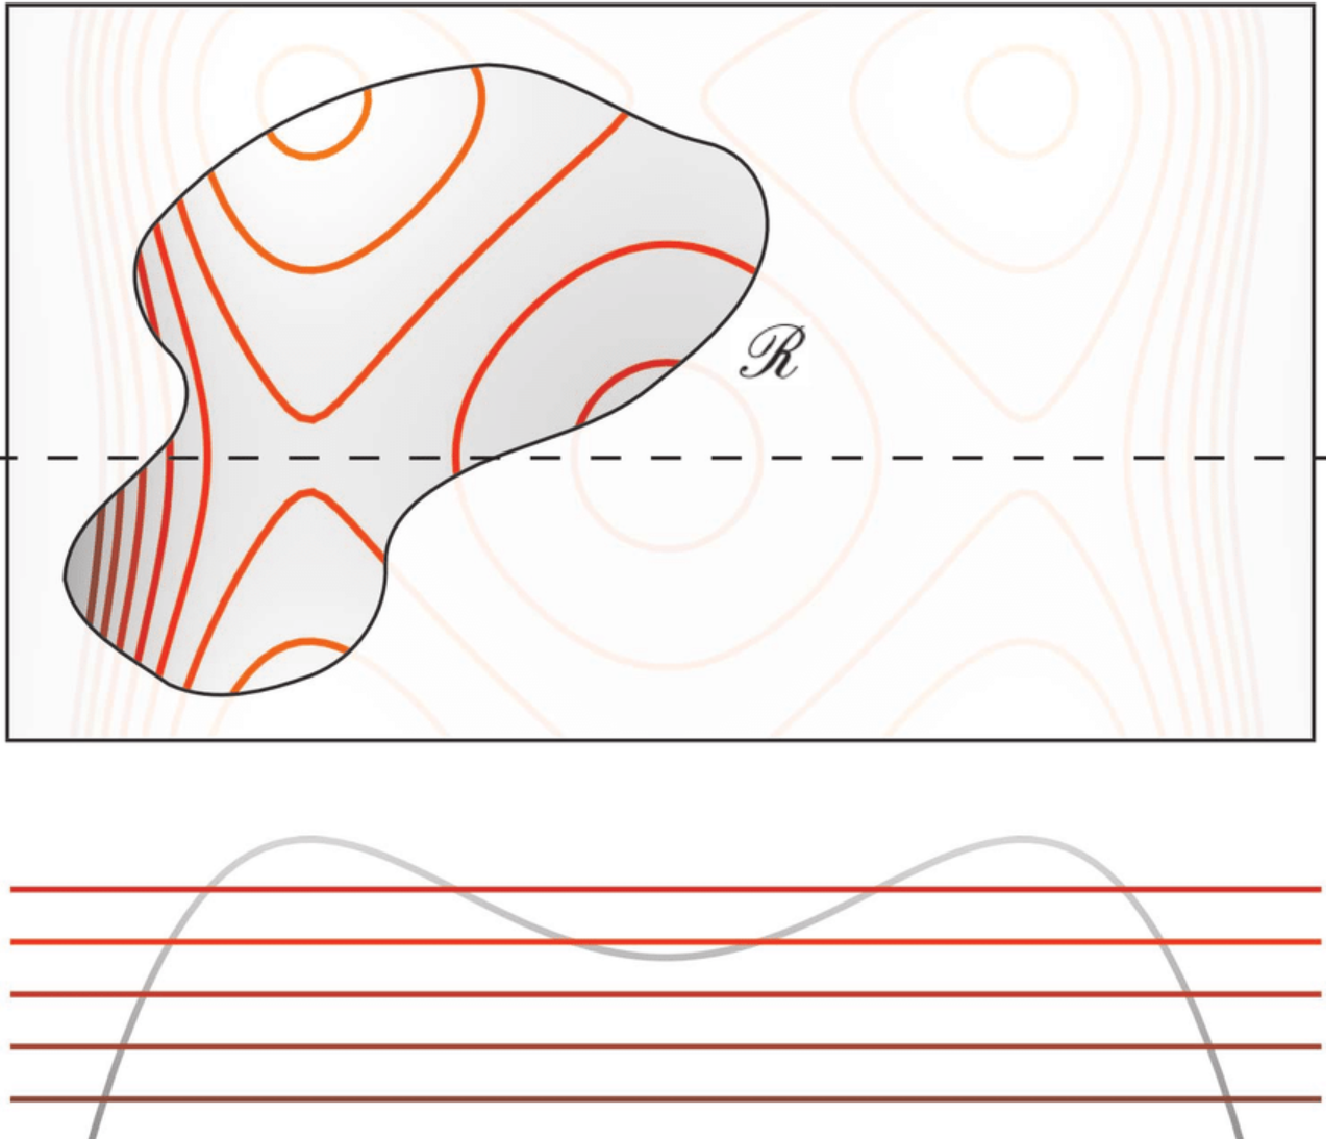
\includegraphics[scale=0.3]{figures/Coarea.pdf}
\end{figure}

Bereits die Definition der beschränkten Variation ([\ref{def2.14}, Definition 2.14]) erinnert teilweise an die Definition der Sobolevräume. Die Coarea-Formel bestätigt einen weiteren Zusammenhang. Und tatsächlich findet man auch einen allgemeinen Zusammenhang zu den Sobolevräumen - wir werden darauf in \ref{subsec:consobo} näher eingehen. An dieser Stelle noch zur Vervollständigung die bekannten isoperimetrischen Ungleichungen:\\[0.5cm]
\pgfsetfillopacity{0.1}\colorbox{generalYellow}{\begin{minipage}{16cm}{\textcolor{black}{\pgfsetfillopacity{1}}{\label{theo2.21}}}
\textbf{Satz 2.21 (Isoperimetrische Ungleichungen, Notation aus \cite{EvansMeaTh}[Seite 190-192: Theorem 2]):} Sei E eine beschränkte Teilmenge des \(\mathbb{R}^n\) mit endlichem Perimeter. Dann gilt:
\begin{enumerate}
    \item \(\lambda^n(E)^{1-\frac{1}{n}} \leq C_1 |D \chi_E|\),
    \item \(\min \{\lambda^n(\overline{B_{\epsilon}(x)} \, \cap \, E), \, \lambda^n(\overline{B_{\epsilon}(x)} \, \textbackslash \, E)\}^{1-\frac{1}{n}} \leq 2C_2 |D \chi_{\Ball \subset E}|.\)
\end{enumerate}
\end{minipage}}\\

\textsc{Beweis:} Die Aussagen folgen direkt aus den Sobolev-/Poincaré-Äquivalenten für \(\mathcal{BV}\)-Funktionen:
\begin{enumerate}
    \item \(\exists C_1 > 0 \, \forall f \in \mathcal{BV}(\mathbb{R}^n): \, ||f||_{L^{\frac{n}{n-1}}(\mathbb{R}^n)} \leq C_1 |Df|(\mathbb{R}^n)\),
    \item \(\exists C_2 > 0 \, \forall f \in \mathcal{BV}_{\text{loc}}(\mathbb{R}^n): \, ||f - \int_{\overline{\Ball}}f \, d\lambda^n(y)||_{L^{\frac{n}{n-1}}(\overline{\Ball})} \leq C_2 |Df|(\Ball)\),
\end{enumerate}
zusammen mit dem Lemma von Fatou. (Die Konstanten in den isoperimetrischen Ungleichungen stimmen dementsprechend dann auch mit denen aus den Äquivalenten überein.)\QEDB

\subsection[Struktur von BV]{Struktur von \(\mathcal{BV}\)}{\label{subsec:bvstruc}}
In \eqref{eq2.23} hatten wir angemerkt, dass wir für die Gleichheit den Rand von E im Allgemeinen stärker regularisieren müssen. Das zugehörige Theorem stammt von niemand Geringerem als De Giorgi selbst. Doch zuvor müssen wir für die Formulierung einige Begriffe einführen:\\[0.5cm]
\pgfsetfillopacity{0.1}\colorbox{generalYellow}{\begin{minipage}{16cm}{\textcolor{black}{\pgfsetfillopacity{1}}{\label{def2.22}}}
\textbf{Definition 2.22 (Dichten und Rektifizierbarkeit, Notation aus \cite{BraidesApprox}[Seite 18: Definition 1.54]):} \begin{enumerate}
\item Betrachte eine Borelmenge E. Dann nennen wir x einen Punkt der Dichte t \(:\Leftrightarrow\)
    \begin{equation}
        \lim_{\epsilon \to 0^+} \frac{\lambda^n(E \cap B_{\epsilon}(x))}{\lambda^n(B_{\epsilon}(x))} = t \in [0,1]\text{ existiert.}
    \end{equation}
    Die zugehörige Menge bezeichnen wir mit \(E_t\). 
\item Besitzt E endlichen Perimeter auf A, dann definieren wir den De Giorgi reduzierten Rand von E durch:
\begin{equation}{\label{eq2.28}}
    \partial^* E := \{x \in \text{supp} (|D \chi_E |) \, | \, \exists \lim_{\epsilon \to 0^+} \frac{D \chi_E (B_{\epsilon}(x))}{|D \chi_E|(B_{\epsilon}(x))} =: n(x) : \partial^* E \to \mathbb{S}^{n-1}\},
\end{equation}
wobei n(x) innere Normale an E genannt wird.
\item Eine Teilmenge S des \(\mathbb{R}^n\) nennen wir rektifizierbar, falls eine  \textbf{abzählbare} Familie \((\gamma_i)_{i \in I}\) an Graphen von (n-1)-dimensionalen Lipschitz-Funktionen existiert mit \(\mathcal{H}^{n-1}(S \, \textbackslash \cup_{i=1}^{\infty} \gamma_i) = 0\).
\end{enumerate}
\end{minipage}}\\

\textbf{Bemerkung:} Die Nomenklatur in [\ref{def2.22}, Definition 2.22 (1)] erinnert stark an [\ref{lem2.3}, Lemma 2.3]. Und tatsächlich handelt es sich um eine verstärkte Lebesgue-Maß-Variante für E (aus [\ref{lem2.3}, Lemma 2.3] folgt z.B. direkt, dass \(D \chi_E = n(x) |D \chi_E|\) gilt). Damit ist aber aus diesem Zusammenhang auch sofort klar, dass die Wohldefiniertheit dem Satz von Radon-Nikodym zu entnehmen ist.\\

Bevor wir uns zwei Beispiele anschauen, eine kurze Erinnerung an die Definition einer rektifizierbaren Kurve. Hiermit ist eine \(C^1\)-Kurve gemeint, die stets auf ihre Bogenlänge parametrisiert werden kann. Das ist natürlich möglich, da dank der Stetigkeit der Ableitung der Kurve, die zugehörige Geschwindigkeit ebenfalls stetig ist, weshalb diese \(\mathcal{B}(I)\)-messbar ist, wobei \(I\) hier ein Intervall ist. Graphisch entspricht das folgender Intuition für eine Kurve \(\gamma \in C^1(]a,b[,\mathbb{R}^N)\):
\begin{figure}[label={fig:rectcurve}, caption={Rektifizierung von \(\gamma\) für \(N=1\): Parametrisierung auf Bogenlänge durch Umparametrisierung mit \(\Phi\)}]
  \centering
\begin{tikzpicture}
    \draw[orange, bend left=30] (3,0) to (4,2);
    \draw[->] (5,1) -- (7,1);
    \draw[orange] (8,1) -- (10.7,1);
    \coordinate[label=left:$\gamma(a)$] (a) at (3,0);
    \coordinate[label=left:$\gamma(b)$] (b) at (4,2);
    \coordinate[label=below:$(\gamma \circ \Phi)(a)$] (aa) at (8,1);
    \coordinate[label=below:$(\gamma \circ \Phi)(b)$] (bb) at (10.7,1);
    \fill (a) circle (2pt);
    \fill (b) circle (2pt);
    \fill (aa) circle (2pt);
    \fill (bb) circle (2pt);
    \draw (6,1.5) node {$\Phi$};
\end{tikzpicture}
\end{figure}

Ein Beispiel einer nicht-rektifizierbaren Menge ist alles andere als einfach zu skizzieren. Dies liegt daran, dass kompakte, zusammenhängende Teilmengen des \(\mathbb{R}^n\) mit endlichem \(\mathcal{H}^1\)-Maß \textbf{immer} rektifizierbar sind (intuitiv ist das klar, denn diese Mengen sind folglich das Bild einer rektifizierbaren Kurve; für Details verweisen wir auf \cite{falconer1985geometry}). Wir errinnern an dieser Stelle an das bekannte Fraktal \(\mathcal{C}\), der Cantor-Menge, dessen "nicht-magere" Version wir nun betrachten wollen. Wir entfernen aus dem Einheitsintervall iterativ die "mittlere Hälfte" des jeweiligen Intervalls und nennen die so konstruierte Menge \(\mathcal{C}_{1/2}\). Woran wir letztendlich interessiert sind, ist die Menge \(\mathcal{C}_{1/2} \times \mathcal{C}_{1/2}\), also eine "4-Ecken-Menge". Doch wieso ist diese Menge nun nicht-rektifizierbar? Das Problem ist, dass eine vertikale und horizontale orthogonale Projektion dieser Menge Länge 0 besitzen (klar, denn diese Projektionen entsprechen \(\mathcal{C}_{1/2}\)). Ein beeindruckendes Resultat von Besicovitch besagt, dass in einer Menge im \(\mathbb{R}^2\), die eine derartige Eigenschaft besitzt, \(\lambda^2\)-f.a. Projektionen die Länge 0 besitzen (siehe \cite{bishop2017fractals}[Seite 283 ff.] für einen Beweis). Damit kann die "4-Ecken-Menge" nicht rektifizierbar sein.
\begin{figure}[]
  \begin{subfigure}[t]{.4\textwidth}
  \centering
\begin{tikzpicture}
    \draw [name path = AA, gray] (0,0) -- (4,0);
    \draw [name path = AB, gray] (0,0) -- (0,-4);
    \draw [name path = AC, gray] (4,-4) -- (0,-4);
    \draw [name path = AD, gray] (4,-4) -- (4,0);
    \tikzfillbetween [of=AA and AC]{gray};

    \draw [name path = A, red] (0,0) -- (1,0);
    \draw [red] (0,0) -- (0,-1);
    \draw [red] (1,0) -- (1,-1);
    \draw [name path = B, red] (0,-1) -- (1,-1);
    \tikzfillbetween [of=A and B]{red};
    \draw [name path = C, red] (3,0) -- (4,0);
    \draw [red] (3,0) -- (3,-1);
    \draw [red] (4,0) -- (4,-1);
    \draw [name path = D, red] (3,-1) -- (4,-1);
    \tikzfillbetween [of=C and D]{red};
    \draw [name path = E, red] (0,-3) -- (1,-3);
    \draw [red] (0,-3) -- (0,-4);
    \draw [red] (1,-4) -- (1,-3);
    \draw [name path = F, red] (1,-4) -- (0,-4); 
    \tikzfillbetween [of=E and F]{red};
    \draw [name path = G, red] (3,-3) -- (4,-3);
    \draw [red] (3,-3) -- (3,-4);
    \draw [name path = H, red] (4,-4) -- (3,-4);
    \draw [red] (4,-4) -- (4,-3);
    \tikzfillbetween [of=G and H]{red};

    \draw (-0.3,0) -- (-0.3,-4);
    \draw (0,0.3) -- (4,0.3);
    \coordinate (a) at (0,0);
    \coordinate (b) at (4,0);
    \coordinate (c) at (0,-4);
    
    \node at (a) [above left = 1mm of a] {0};
    \node at (b) [above right = 1mm of b] {1};
    \node at (c) [below left = 1mm of c] {1};
\end{tikzpicture}
\caption*{Eine Iteration der "4-Ecken-Menge"}
\end{subfigure}%
\hfill
\begin{subfigure}[t]{.35\textwidth}
  \centering
  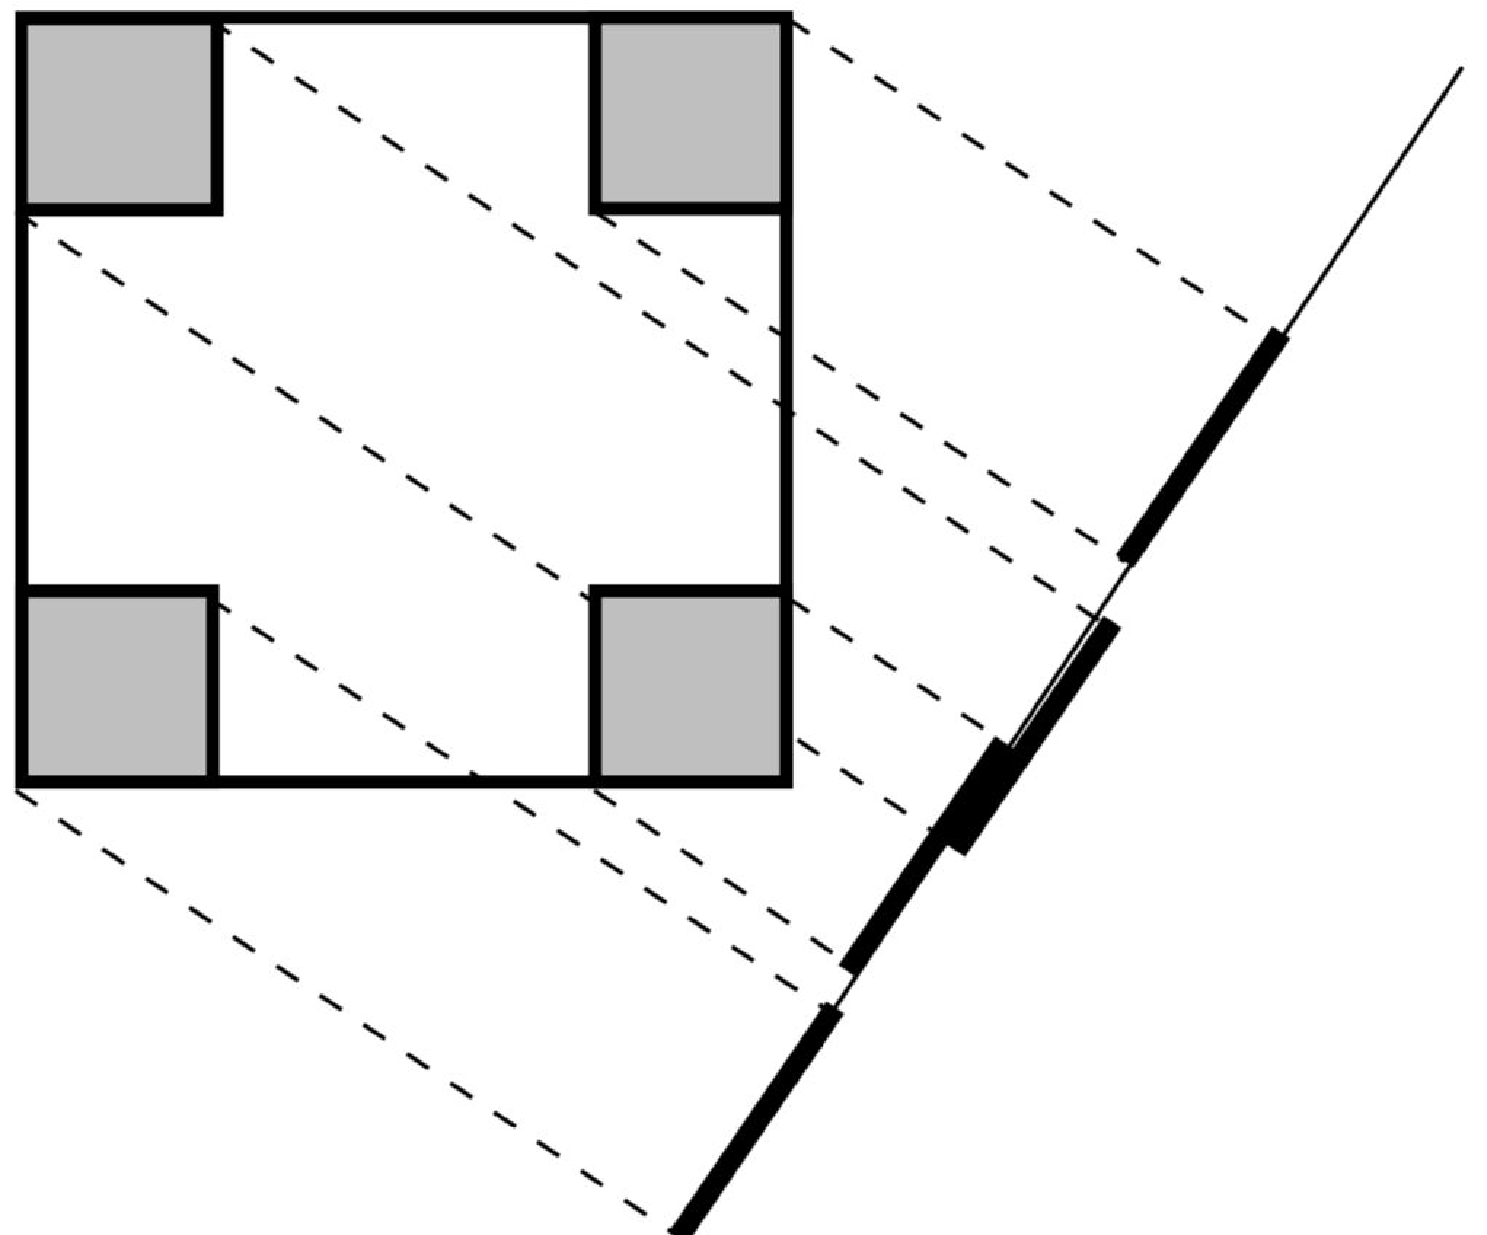
\includegraphics[width=1.0\linewidth]{figures/CorProj.pdf}
  \caption*{Illustration der Projektionen \cite{peres2003fractals}[Seite 318]}
  \label{fig:corproj}
\end{subfigure}%
\end{figure}
\newpage
Nun zu den besagten zwei Beispielen:
\begin{figure}
\centering
\begin{minipage}{.35\textwidth}
  \centering
  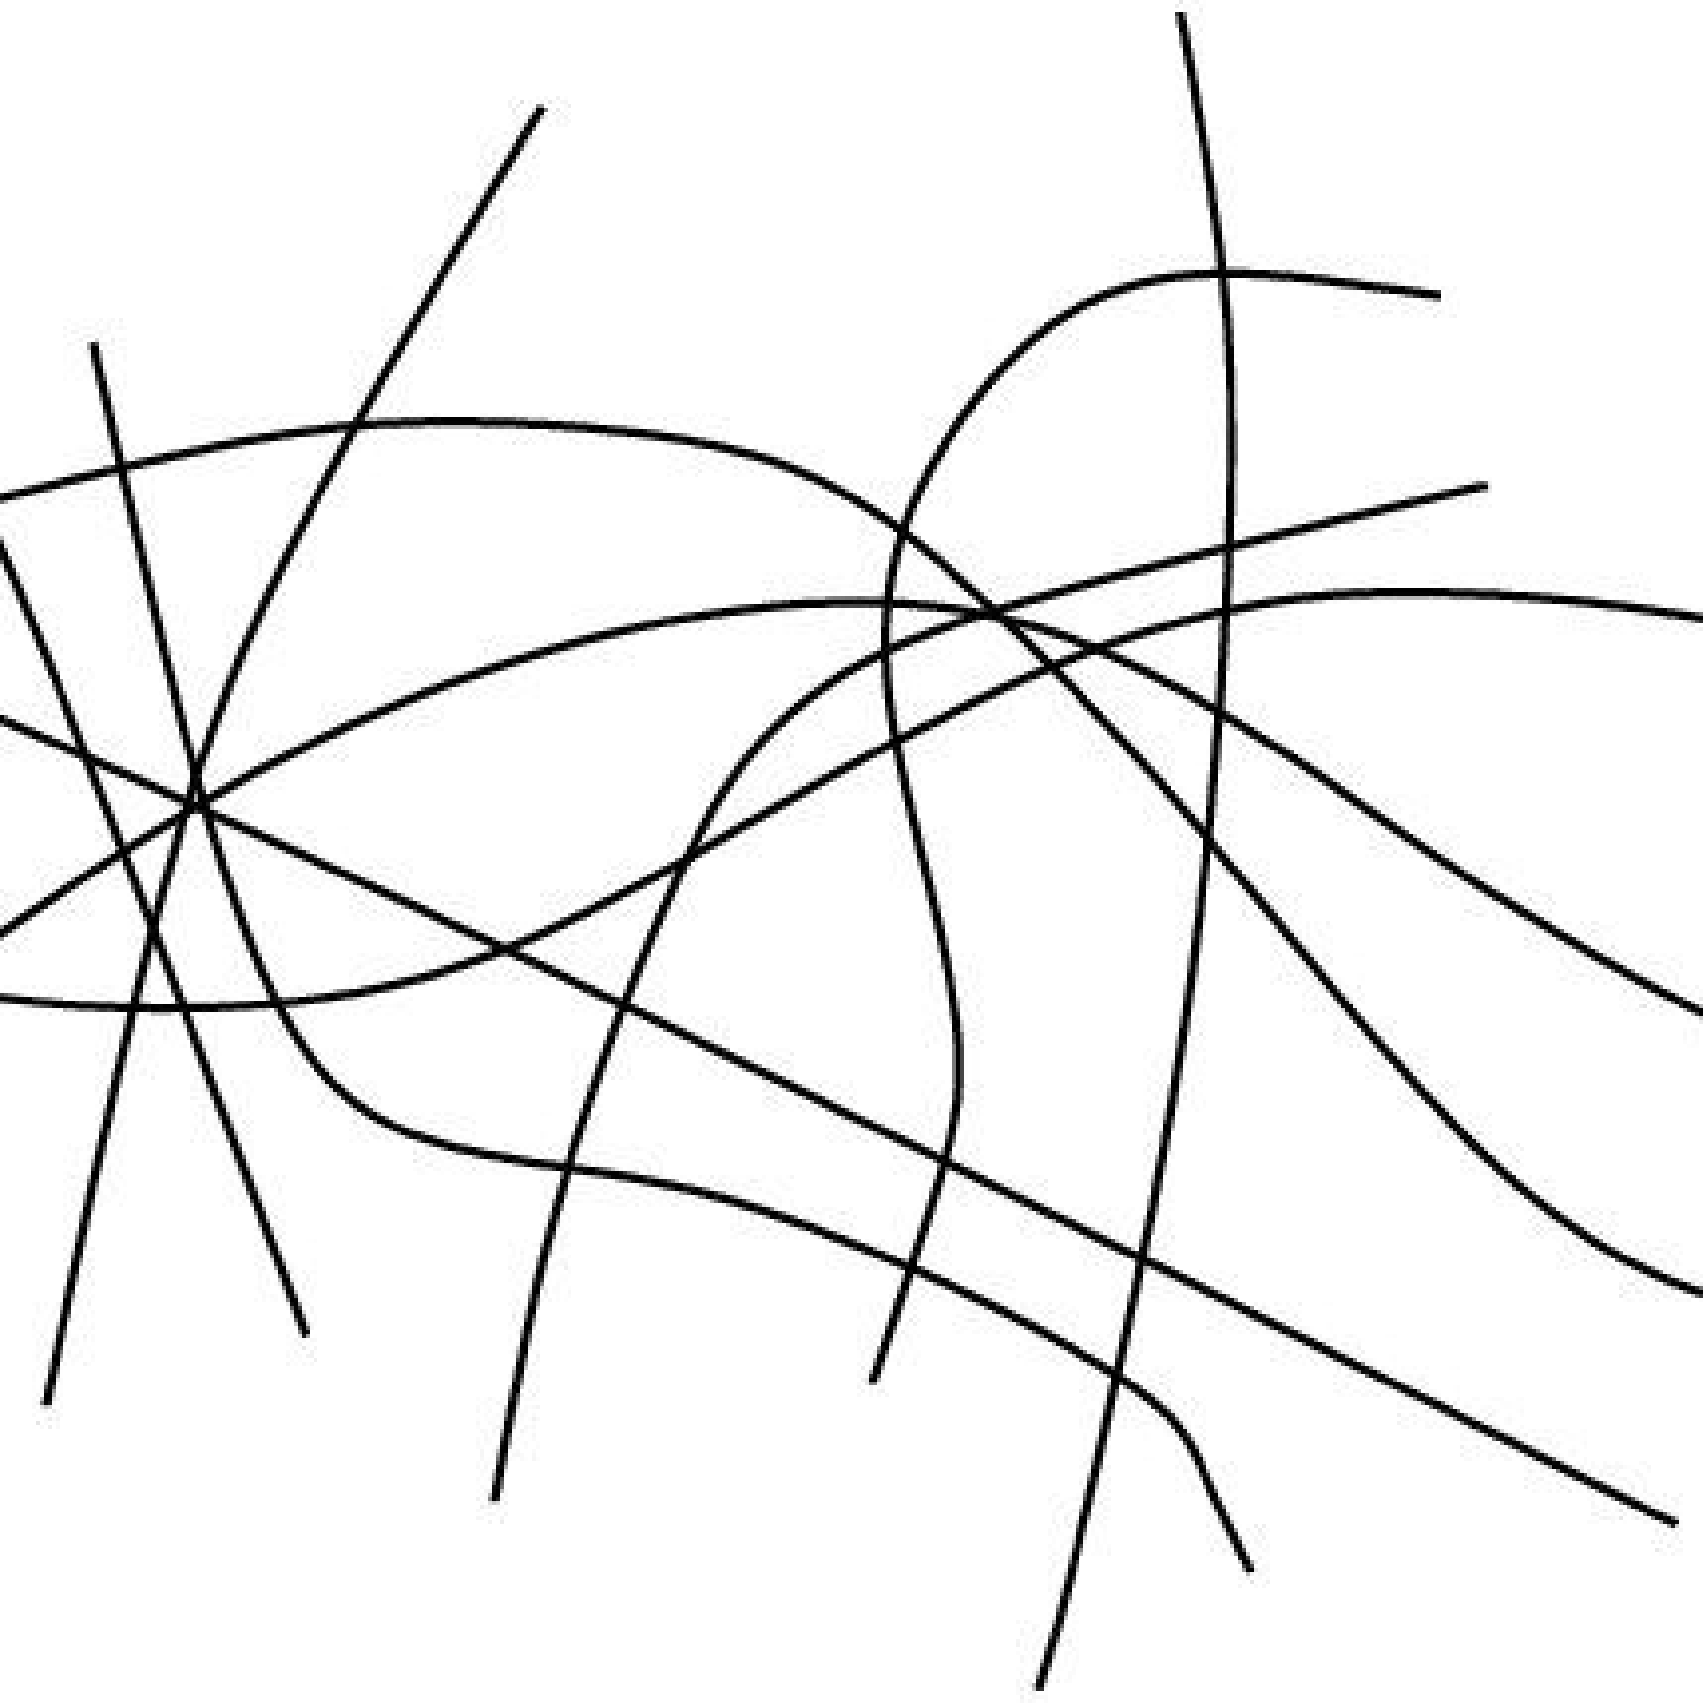
\includegraphics[width=1.0\linewidth]{figures/RectSet.pdf}
  \caption*{Ein Beispiel für eine rektifizierbare Menge \cite{RectCurve}}
  \label{fig:RectCurve}
\end{minipage}%
\(\, \,\)
\begin{minipage}{.35\textwidth}
  \centering
  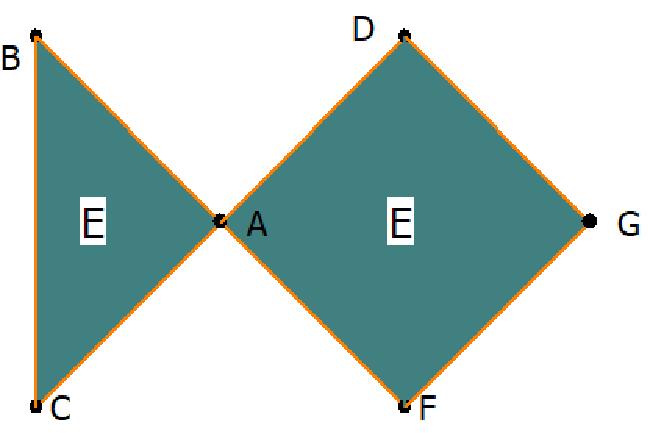
\includegraphics[width=1.5\linewidth]{figures/DeGiorgiRand.pdf} 
  \caption*{Ein Beispiel einer Borelmenge E mit endlichen Perimeter}
  \label{fig:deGiorgiRand}
\end{minipage}%
\end{figure}

Eine rektifizierbare Menge ist also die Verallgemeinerung einer rektifizierbaren \\\(\mathcal{C}^1\)-Kurve, wie mit dem Bild und folgendem Fakt deutlich wird: Reellwertige lipschitz-stetige Funktionen sind f.ü. klassich differenzierbar (Satz von Rademacher, siehe [\ref{theoA.1}, Anhang A.1]). Man kann sogar noch einen Schritt weiter gehen: Im Prinzip sind rektifizierbare Mengen eine Verallgemeinerung von \(C^1\)-Untermannigfaltigkeiten (im \(\mathbb{R}^n\)), zu verstehen in einem maßtheoretischen Kontext.\\
Betrachten wir nun das zweite Beispiel etwas genauer. Wir wählen hier alles andere als zufällig ein \textbf{nicht}-\(C^1\) Beispiel, denn \(C^k\)-Gebiete, wobei \(k \geq 1\), weißen genug Regularität auf, dass dann \(\partial^* E = \partial E\) gilt (folgt direkt aus \eqref{eq2.23} und [\ref{lem2.3}, Lemma 2.3]).\\
Zuerst fällt auf, dass der Punkt A Dichte t=\(\frac{1}{2}\) besitzt, also \(A \in E_{\frac{1}{2}}\), weshalb \(E_{\frac{1}{2}} = \partial E \, \textbackslash \, \{B,C,D,F,G\}\) gilt. Damit wird klar: Die Bedingung für \(E_t\) ist ein Relativmaß dafür, wie dicht ein Punkt x in der Menge E liegt. Es ist dann naheliegend, dass man allgemein \(E_1\) die Menge der "Dichtepunkte" von E nennt. Zusätzlich bemerken wir noch, dass \(\text{supp} (|D \chi_E |) = \partial E\), sowie \(\partial^* E = \partial E \, \textbackslash \, \{A,B,C,D,F,G\}\) gilt, da der Limes aus [\ref{def2.22}, Definition 2.22 (2)] in den "Eckpunkten" nicht in \(\mathbb{S}^1\) liegt.\\ \textit{Beweis: o.B.d.A. sei \(D=(0,0)\) (dank der Translationsinvarianz des Lebesgue-Maßes). Dann ist \(D\chi_E (B_{\epsilon}(D)) = (\epsilon,\epsilon)\). Es folgt, dass \(||n(D)||_{ecl} = \frac{1}{\sqrt{2}}\) ist. Analog für \(A,B,C,F,G\) (für alle anderen Punkte von \(\partial E\) ist aufgrund der \(C^1\)-Regularität nichts zu zeigen nach obiger Bemerkung) \QEDB}\\
Allgemein lässt sich zeigen (siehe z.B. \cite{maggi2012sets}[Seite 170: Corollary 15.8]), dass \(\partial^* E \subset E_{\frac{1}{2}}\) gilt.\\

Nach dieser Illustration nun zu dem besagten Theorem:\\[0.5cm]
\pgfsetfillopacity{0.1}\colorbox{generalYellow}{\begin{minipage}{16cm}{\textcolor{black}{\pgfsetfillopacity{1}}{\label{theo2.23}}}
\textbf{Satz 2.23 (Rektifizierbarkeitssatz von De Giorgi, Notation aus \cite{BraidesApprox}[Seite 18: Theorem 1.55]):} Sei E eine Teilmenge des \(\mathbb{R}^n\) mit endlichen Perimeter auf A, B eine Borelmenge und Teilmenge von A. Dann gilt:
\begin{enumerate}
    \item \(\partial^* E\) ist rektifizierbar.
    \item \(|D \chi_E|(B) = \mathcal{H}^{n-1}(B \cap \partial^* E)\).
    \item \(\mathcal{H}^{n-1}(\partial^* E) < \infty\).
    \item \(\mathcal{H}^{n-1}(A \, \textbackslash \, E_0 \cup \partial^* E \cup E_1)) = \mathcal{H}^{n-1}(A \cap (\partial^* E \Delta E_{\frac{1}{2}})) = 0\).
    \item die verallgemeinerte Greensche Formel:
    \begin{equation}
        \int_E \text{div }f \, d\lambda^n(x) = - \int_{\partial^* E} <\text{n},f>_{\mathbb{R}^n} \, d\mathcal{H}^{n-1} \, \, \forall f \in \mathcal{C}^1_c(A,\mathbb{R}^n),
    \end{equation}
\end{enumerate}
wobei n die innere Normale an E ist.
\end{minipage}}\\

\textsc{Beweis:} Der Beweis von (1), (2) und (4) ist äußerst aufwändig, weshalb wir auf \cite{DeGiorgiRecTheorem} für (2) und auf H. Federer's Werke \cite{federer1947k} bzw. \cite{federer2014geometric} für (1) und (4) verweisen. Des Weiteren ist (3) eine direkte Konsequenz aus (2) und (5) folgt direkt aus der zugehörigen Radon-Nikodym-Ableitung, \eqref{eq2.28} und (2).\QEDB

\subsection[Nutzen für die Gamma-Konvergenz]{Nutzen für die \(\Gamma\)-Konvergenz}{\label{subsec:gammabvuse}}
Um das Konzept der \(\Gamma\)-Konvergenz in den folgenden Kapiteln besser zu verstehen, betrachten wir nun approximative Stetigkeit und Differenzierbarkeit. Diese beiden Begriffe werden auf die eigentliche Natur von \(\mathcal{BV}\)-Funktionen führen.\\[0.5cm]
\pgfsetfillopacity{0.1}\colorbox{generalYellow}{\begin{minipage}{16cm}{\textcolor{black}{\pgfsetfillopacity{1}}{\label{def2.24}}}
\textbf{Definition 2.24 (Approximative Eigenschaften):} Betrachte eine Borelmenge A als Teilmenge des \(\mathbb{R}^n\) und eine skalare Funktion \(u:A \to \mathbb{R}\). Dann seien für \(x \in A\) definiert:
\begin{itemize}
    \item \(u^+ := ap-\limsup_{y \to x} u(y) := \inf \{t \, | \, \{u > t\} \text{ hat Dichte 0 in x}\}\),
    \item \(u^- := ap-\liminf_{y \to x} u(y) := \sup \{t \, | \, \{u > t\} \text{ hat Dichte 1 in x}\}\),
    \item \(J(u) := \{x \in A \, | \, u^- \text{ existiert nicht.}\}\).
\end{itemize}
Ist nun \(x \in A \, \textbackslash \, J(u)\), so nennt man x approximativ differenzierbar, falls ein \(\xi \in \mathbb{R}^n\) existiert, sodass gilt:
\begin{equation}
    ap-\lim_{y \to x} \frac{|u(y) - v(x) - <\xi,y-x>|}{|y-x|} = 0 \, \, \forall v:J(u) \to \mathbb{R}.
\end{equation}
\end{minipage}}\\

\textbf{Bemerkung:} \begin{itemize}
    \item \(\xi\) wird in diesem Fall als approximativer Gradient von x bezeichnet. Allgemein erinnert die Defintion ein wenig an den Subgradienten, weshalb wir diesen hier noch einmal aufführen:\\
    Sei \((\mathcal{X},||\cdot||)\) ein Banachraum, \(\mathcal{F}:\mathcal{X} \to \overline{\mathbb{R}}\). Dann nennen wir \(x^* \in \mathcal{X}^*\) den Subgradienten von \(\mathcal{F}\) in \(x \in \mathcal{X}\), falls  gilt:
    \begin{equation}{\label{eq.2.31}}
        \mathcal{F}(y) \geq \mathcal{F}(x) + <x^*,y-x> \, \, \forall y \in \mathcal{X}.
    \end{equation}
    \item Die Menge J(u) nennt man auch Menge der "Sprungpunkte" (von u).
\end{itemize}

Um mithilfe der definierten Approximationen die Struktur von \(\mathcal{BV}\)-Funktionen mathematisch besser fassen zu können, führen wir hier eine weitere Konsequenz des Radon-Nikodym Theorems auf:\\
Dazu erinnern wir an die Maßtheorie, aus der wir wissen, dass wir den singulären Anteil der Radon-Nikodym-Zerlegung für ein Maß \(\mu\) eines \(\sigma\)-endlichen Maßraum \((A,\Sigma_A,\mu)\) (unter natürlich passenden Voraussetzungen) weiter zerlegen können in:
\begin{equation}
    \mu_s = \mu_p + \mu_{sc},
\end{equation}
wobei \(\mu_p\) den Punktanteil und \(\mu_{sc}\) den singulär-stetigen Teil bezeichnet. Wir definieren also für \(u \in \mathcal{BV}(A,\mathbb{R}^N)\) die Zerlegung von \(Du\) in:
\begin{equation}
    Du = D^a u + D^j u + D^c u,
\end{equation}
wobei \(D^a u\) den absolut stetigen Anteil von \(Du\), \(D^j u := \chi_{J(u)} \cdot Du\) den Sprunganteil von \(Du\) und \(D^c u := \chi_{A \textbackslash J(u)} \cdot D^s u\) den Cantoranteil von \(Du\) darstellen (Bemerkung: Nach Definition sind folglich \(D^a u, \, D^j u \text{ und }D^c u\) paarweise singulär zueinander.). Im Folgenden wird für die Struktur vor allem die Darstellung von \(D^j u\) entscheidend sein, weshalb wir diese nun charakterisieren werden:\\[0.5cm]
\pgfsetfillopacity{0.1}\colorbox{generalYellow}{\begin{minipage}{16cm}{\textcolor{black}{\pgfsetfillopacity{1}}{\label{theo2.25}}}
\textbf{Satz 2.25 (Darstellung des Sprunganteils):} Sei \(u \in \mathcal{BV}(A,\mathbb{R}^N)\). Dann ist J(u) rektifizierbar und es gilt:
\begin{equation}
    D^j u = (u^+ - u^-) \otimes n_u \chi_{J(u)} \cdot \mathcal{H}^{n-1}(A).
\end{equation} 
\end{minipage}}\\

\textsc{Beweis:} Betrachte \(E(t) := \{u > t\}, \, J_t := A \, \textbackslash \, (E(t)_0 \cup E(t)_1)\). Wir nutzen nun [\ref{theo2.23}, Satz 2.23 (1)] und sehen, dass \(J_t\) rektifizierbar ist (falls E(t) endlichen Perimeter besitzt; diese Annahme ist nicht restriktiv, da wir mithilfe von [\ref{theo2.20}, Satz 2.20] die Annahme im Zweifel für eine abzählbar dichte Menge in \(\mathbb{R}\) erhalten.). Mithilfe der approximativen Stetigkeit erhalten wir dann daraus auch die Rektifizierbarkeit von J(u). Die zweite Aussage folgt direkt aus einer Anwendung von [\ref{theo2.20}, Satz 2.20] und [\ref{theo2.23}, Satz 2.23]. Für weitere Details verweisen wir auf \cite{BraidesApprox}[Seite 20].\QEDB
\subsection{Zusammenhang zu Sobolevräumen}{\label{subsec:consobo}}
Wenn man das erste Mal auf Sobolevfunktionen stößt, könnte man den Eindruck bekommen, diese wären Funktionen, die eine klassische Ableitung f.ü. besitzen und damit aber schwach differenzierbar sind, da dies im Integral-Sinne keinen Unterschied macht. Diese Vorstellung ist aber nicht ganz korrekt, wie die Signumsfunktion beispielsweise zeigt. Diese weist die wahre Charakterisierung auf: Die eben genannte Beschreibung trifft zu für Sobolevfunktionen unter der zusätzlichen Annahme, dass die Funktion \text{nicht} "springt", also auf einer Nullmenge niederer Dimension nicht-stetig fortsetzbar ist.\\
Diese stärkere Regularität entfernt der Raum \(\BV\). Hier werden genau diese Funktionen zugelassen, i.e. die erstgenannte Vorstellung war in Wahrheit die von \(\mathcal{BV}\)-Funktionen. Zur Illustration betrachten wir folgendes Beispiel:\\
\textbf{Beispiel:} Betrachte folgende Treppenfunktion:
\begin{equation}
    H(x) := \chi_{[a,\infty[}(x) := \begin{cases} 0, \, x < a \\ 1, \, x \geq a \end{cases},
\end{equation}
wobei \(H : \mathbb{R} \to \mathbb{R}\). Dann ist die distributionelle Ableitung von \(H\) das Dirac-Maß \(\delta_a\). Damit ist klar: \(H \in \mathcal{BV}(\mathbb{R})\), aber \(H \notin W^{1,1}(\mathbb{R})\).\\

Diese Diskussion kann man noch deutlich mehr präzisieren. So gilt z.B. allgemein \(W^{1,1}(\mathbb{R}) \subset \mathcal{BV}(\mathbb{R})\). Intuitiv entspricht die \(\mathcal{TV}\)-Halbnorm "im Limes" der Sobolev-Norm. Für mehr Details hierzu verweisen wir auf \cite{BVSobolev}.